\documentclass{beamer}
%\documentclass[handout]{beamer}

\mode<presentation>
{% AnnArbor
%\usetheme{AnnArbor}
  %\usetheme{Boadilla}
  \usetheme{CambridgeUS}
 %\usetheme{Madrid}
  \setbeamercovered{transparent}
}

\usepackage{fontspec,xltxtra,xunicode,moreverb}

\usepackage[french]{babel}
% \usepackage{beamerthemesplit} // Activate for custom appearance

%% No navigation symbol.
\setbeamertemplate{navigation symbols}{}
\beamertemplatenavigationsymbolsempty

%\setbeameroption{hide notes}

% \newcommand{\mypause}{\pause}
\newcommand{\mypause}{~}

\newcommand{\mypauseBeforeExercise}{\pause}

\newcommand{\elvrm}{\rm}
\newcommand{\fivrm}{\rm}
\newcommand{\sixrm}{\rm}
\newcommand{\sevrm}{\rm}
\newcommand{\egtrm}{\rm}
\newcommand{\ninrm}{\rm}
\newcommand{\tenrm}{\rm}
\newcommand{\twlrm}{\rm}
\newcommand{\frtnrm}{\rm}
\newcommand{\svtnrm}{\rm}
\newcommand{\twtyrm}{\rm}
\newcommand{\twfvrm}{\rm}

\newcommand{\ex}{{\bf Exemple}}
\newcommand{\afor}{\bf for}
\newcommand{\ato}{\bf to}
\newcommand{\ado}{\bf do}
\newcommand{\aendo}{\bf endo}
\newcommand{\esp}{\hspace{0.5cm}}

\newcommand{\sal}{\sum_i \mu_i}
\newcommand{\sbet}{\sum_j \nu_j}
\newcommand{\If}{\mbox{\bf if }}
\newcommand{\Then}{\,\mbox{\bf then }}
\newcommand{\titre}[1]{\title{{{\color{red} \large \bf #1}}}}

% Needed for course 2.
\newcommand{\Zn}{{\bf Z}^n}
\newcommand{\Z}{{\bf Z}}
\newcommand{\N}{{\bf N}}
\newcommand{\Np}{{\bf N}^p}

\newcommand{\alfa}{\textsc{alpha}}
\newcommand{\alfacase}{\mbox{\bf case}}
\newcommand{\alfaesac}{\mbox{\bf esac}}
\newcommand{\zset}{\mathbb{Z}}

\newcommand{\sys}{{\bf system}}
\newcommand{\real}{{\bf real}}
\newcommand{\of}{{\bf of}}
\newcommand{\lett}{{\bf let}}
\newcommand{\tel}{{\bf tel}}
\newcommand{\returns}{{\bf returns}}
\newcommand{\boolean}{{\bf boolean}}
\newcommand{\true}{{\bf true}}
\newcommand{\false}{{\bf false}}

\newcommand{\pomme}{\texttt{cmd}}
\newcommand{\alalign}{{$\hookleftarrow$}}

\newcommand{\pyth}{{\sc Python}}
\newcommand{\prog}[1]{\alert{\texttt{#1}}}

\title{Introduction à l'informatique, avec \pyth{}}
% \author{Patrice Quinton}
\author{Lilian Besson}
\date{2020--2021\\Version du \today}

\institute% (optional, but mostly needed)
{ENS Rennes}

\date%[\today] % (optional, should be abbreviation of conference name)
[Info -- DEM - 2020]{Initiation à l'informatique -- DEM -- 2020\\Module 3}
\logo{
\includegraphics[height=0.5cm]{logoENS.pdf}}

% Delete this, if you do not want the table of contents to pop up at
% the beginning of each subsection:
\AtBeginSection[]
{
  \begin{frame}<beamer>
    \frametitle{Plan du cours}
%    \tableofcontents[currentsection,currentsubsection]
\tableofcontents[currentsection,currentsubsection,hideallsubsections]
  \end{frame}
}

\begin{document}

\frame{\titlepage}

\section[Outline]{}
\frame{\tableofcontents}
\frame{
\frametitle{\emph{``Résumé des épisodes précédents''}}
% {\footnotesize
On a vu:
  \begin{itemize}
  \item ce qu'est un algorithme
  \item comment accéder à l'ordinateur via son \prog{terminal}
  \item quelques commandes simples permettant de se déplacer dans la \prog{hiérarchie des fichiers} (\prog{cd}, \prog{ls}, etc)
  \item comment démarrer \pyth{}
  \item comment écrire un programme avec l'éditeur \prog{idle}
  \item les \prog{variables}, leur \prog{type}, l'affectation etc.
  % \item la boucle \prog{while},
  \end{itemize}
La suite : \prog{instructions conditionnelles}, \prog{boucles répétitions}
% }
}

\section{Conditions, instructions conditionnelles}

\frame{
\frametitle{Conditions}\mypause{}
\footnotesize{
\begin{itemize}
\item On peut définir des expressions dont la valeur est \prog{True} (vrai)
ou \prog{False} (faux)\mypause{}
\item On appelle ces expressions des \alert{expressions booléennes} (du nom
du mathématicien Boole) ou encore des \alert{expressions conditionnelles}
ou encore plus simple, des \alert{conditions}\mypause{}
\item Le type des expressions conditionnelles est \prog{bool}\mypause{}
\item Les opérateurs de comparaison (\prog{>, >=, ==, !=, <, <=}) permettent
de former des expressions conditionnelles\mypause{}
\item Si \prog{e} et \prog{f} sont des expressions conditionnelles,
\begin{itemize}
\item \prog{e and f} est l'expression conditionnelle qui est vraie (\prog{True}) si
\prog{e} et \prog{f} sont vraies, sinon elle est fausse (\prog{False})\mypause{}
\item \prog{e or f} est l'expression conditionnelle qui est vraie si l'une des
expressions \prog{e} ou \prog{f} est vraie, fausse sinon\mypause{}
\item \prog{not e} est l'expression conditionnelle qui est vraie si
\prog{e} est fausse et inversement
\end{itemize}
\end{itemize}
}
}



\frame{
\frametitle{Instruction conditionnelle}
\begin{block}{\prog{if}}\mypause{}
L'instruction \prog{if} prend la forme suivante:\\
\prog{
\begin{tabular}{l}
if condition:\\
\hspace{0.5cm} instruction1\\
else:\\
\hspace{0.5cm} instruction2
\end{tabular}
}
\end{block}

\begin{itemize}
\item \prog{condition} est une expression conditionnelle\mypause{}
\item \prog{instruction1} est une instruction qui sera exécutée si
la condition est vraie (\prog{= True})\mypause{}
\item \prog{instruction2} est une autre instruction qui sera exécutée
si la condition est fausse (\prog{= False})\mypause{}
\item Attention : respectez la présentation de cette instruction, où les
instructions sont {\em décalées} par une tabulation, ou des espaces (convention = nombre multiple de 4)
\end{itemize}
}

\frame{
\frametitle{Instruction conditionnelle}
{\footnotesize
\begin{block}{Exemple}
\prog{
\begin{tabular}{l}
y = -2  ~ \# \emph{on va calculer $|y|$ la valeur absolue de $y$}\\
\texttt{if} y < 0\texttt{:}\\
\hspace{0.5cm} valeur\_absolue\_y = -y\\
\texttt{else :}\\
\hspace{0.5cm} valeur\_absolue\_y = y
\end{tabular}
}
\end{block}
\mypause{}
\begin{block}{Explications}
\begin{itemize}
\item On affecte la valeur \prog{-2} à \prog{y}\mypause{}
\item On exécute l'instruction conditionnelle (\prog{if: ...})\mypause{}
\item La condition est \prog{y < 0} qui est vraie (\prog{True})\mypause{}
\item Donc, on exécute la première {\em branche} de l'instruction conditionnelle (le cas ``si'', \prog{if})
qui donne à \prog{valeur\_absolue\_y} la valeur \prog{-y}, cad, \prog{-(-2) = 2}
\item \emph{Autre exemple} : si \prog{y = 2} au lieu de \prog{y = -2}, la deuxième branche (le cas ``sinon'', \prog{else}) donnerait \prog{valeur\_absolue\_y = y}.
\end{itemize}
\end{block}
}

}

\frame{
\frametitle{Exercice M3.1}
{\footnotesize
\begin{block}{Faire}
\'Ecrire un programme qui demande de deviner un nombre compris entre 1 et 10, et
imprime gagné, trop petit, ou trop grand.

On a besoin pour cela de l'instruction \prog{input("Chaîne de caractères")}.
\prog{\\
  x = int( input( "Donne moi un nombre : "))\\
  }
lit un nombre (sous forme d'une chaîne de caractères) avec \prog{input("...")}, et le convertit en entier (\prog{int(...)}).
\end{block}

\mypauseBeforeExercise{}
\begin{block}{Solution}
  \vspace*{-20pt}
\prog{
\verbatiminput{../Programmes-Python/M3-1.py}
}
\end{block}
}
}

\frame{
\frametitle{Exercice M3.1}
{\footnotesize
\begin{block}{Faire}
\'Ecrire un programme qui demande de deviner un nombre compris entre 1 et 10, et
imprime gagné, trop petit, ou trop grand.

On a besoin pour cela de l'instruction \prog{input("Chaîne de caractères")}.
\prog{\\
    x = int( input( "Donne moi un nombre : "))\\
}
lit un nombre (sous forme d'une chaîne de caractères) avec \prog{input("...")}, et le convertit en entier (\prog{int(...)}).
\end{block}

\mypauseBeforeExercise{}
\begin{block}{Solution}
  \vspace*{-20pt}
\prog{
\verbatiminput{../Programmes-Python/M3-1-2.py}
}
\end{block}
}
}

\section{Itérations: la boucle}

\begin{frame}[fragile]
\frametitle{La boucle ``tant que'' (\prog{while})}
\begin{block}{Instruction \prog{while}}
  \prog{
\begin{tabular}{l}
avant\\
\prog{while} condition:  \# tant que condition est \prog{True}:\\
    \hspace{0.5cm} \# indentation pour délimiter le bloc\\
    \hspace{0.5cm} instructions\\
après
\end{tabular}
  }
  \mypause{}
  \begin{itemize}
    \item
    commence par \prog{avant} (zéro, une ou plusieurs lignes),\mypause{}
    \item
    répète \prog{instructions} tant que la \prog{condition} est vraie (\prog{= True}),\mypause{}
    \item
    puis continue par \prog{après} (zéro, une ou plusieurs lignes).
  \end{itemize}
\end{block}
\end{frame}

\frame{
\frametitle{Exercice M3.2}
{\footnotesize
\begin{block}{Faire}
Avec une boucle \prog{while}, écrire un programme calcule la somme des $n$ premiers nombres entiers :
\prog{somme = 1 + 2 + ... + n}

NB: pour arrêter un programme Python qui boucle, il faut l'interrompre en tapant \prog{control + c}.
\end{block}
\mypauseBeforeExercise{}
\begin{block}{Solution}
\prog{
\verbatiminput{../Programmes-Python/M3-2.py}
}
\end{block}
}
}

\section{Chaînes de caractères}

\frame{
\frametitle{Chaînes de caractères ({\em string})}
{\footnotesize
\begin{block}{Par des exemples}
\begin{itemize}
\item \prog{\texttt{'Ceci est une chaîne'}} est une chaîne de caractères\mypause{}
\item \prog{\texttt{''}} aussi (c'est la \alert{chaîne vide})\mypause{}
\item \prog{\texttt{'Ceci' + ' ' + 'est'}} est la chaîne obtenue en \alert{concaténant}
les trois chaînes \prog{\texttt{'Ceci'}}, \prog{\texttt{' '}} et \prog{\texttt{'est'}} \mypause{}
\item La longueur d'une chaîne est donnée par la fonction \prog{\texttt{len}}\mypause{}
\item \prog{\texttt{machaine[i]}} donne la chaîne formée du $i^{eme}$ caractère
de \prog{machaine} (le premier caractère est numéroté \texttt{0}, le dernier \prog{len(machaine) - 1}).
\item On peut transformer des objets en chaînes de caractères:
\prog{\texttt{str(23)}} est la chaîne obtenue par conversion en chaîne de
l'entier \texttt{23}
\item On peut utiliser \prog{"} comme délimiteur, à la place de \prog{'}, ce qui
  permet d'avoir \prog{'} dans une chaîne.
\end{itemize}
\end{block}
}
}


\frame{
\frametitle{Exercice M3-3}
{\footnotesize
\begin{block}{Faire}
\'Ecrire un programme qui compte le nombre de caractères \texttt{e} dans une
phrase.

\end{block}

\mypauseBeforeExercise{}
\begin{block}{Solution}
\prog{
\verbatiminput{../Programmes-Python/M3-3.py}
}
\end{block}
}

\mypause{}
Culture générale : connaissez-vous ``\emph{La Disparition}'' de Georges Perec ?
}


\section{Conclusion}
\frame
{
\frametitle{En résumé}
\begin{itemize}
\item Vous avez eu un second contact avec \alert{\pyth{}} et son éditeur \alert{\texttt{idle}}\mypause{}
\item Vous avez écrit des programmes, avec des variables,\mypause{}
\item Vous avez manipulé des variables booléennes (\prog{True}/\prog{False}), des conditions
\item et aussi des instructions conditionnelles (\prog{if c: ... elif c2: ... else: ...})\mypause{}
\item et des boucles (\prog{while c: ...})\mypause{}
\item et aussi des chaînes de caractères (type \prog{str})

\item[$\rightarrow$] Module 4 : on continue \pyth{}, en apprenant les \alert{listes} et les \alert{fonctions} !
\end{itemize}
}


\section{Petite histoire : Alan Turing}
\frame
{
\frametitle{Alan Turing : un grand scientifique, un héros de guerre reconnu 50 ans après sa mort}
\vspace*{5pt}
\begin{figure}
  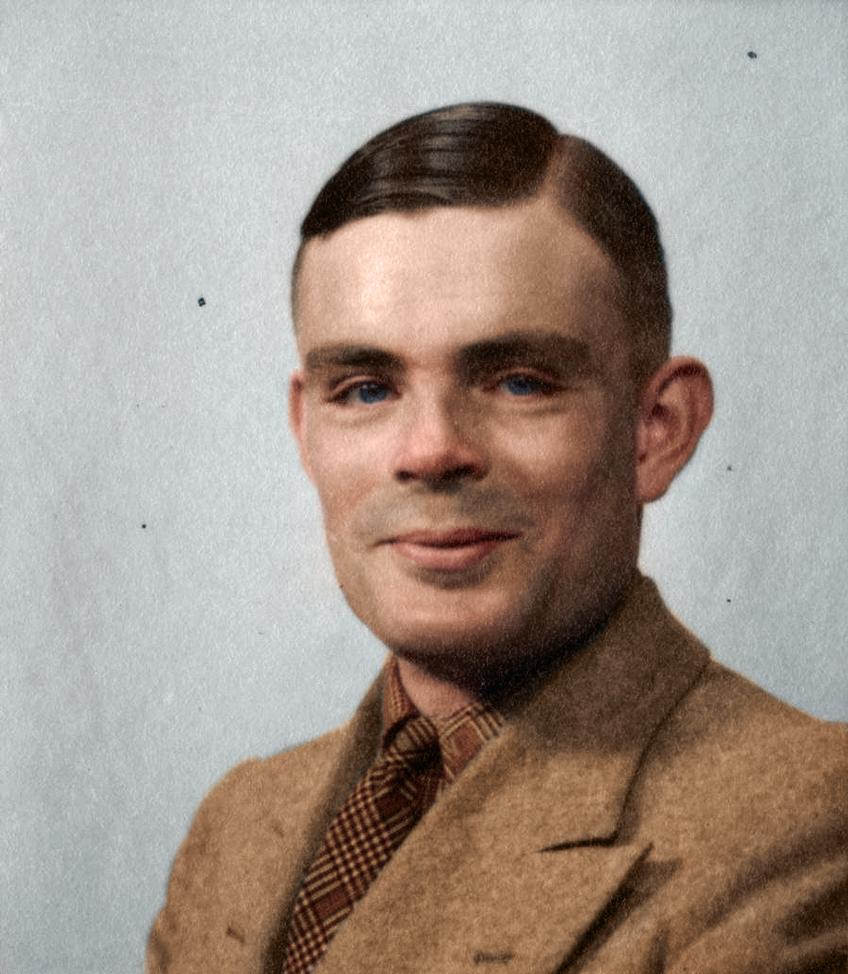
\includegraphics[height=100pt]{Alan_Turing_colorized.jpg}
\end{figure}
\begin{itemize}
  \item Alan Turing, né en 1912 à Londres et mort en juin 1954, est un mathématicien et cryptologue britannique, auteur de travaux qui fondent scientifiquement l'informatique
  \item Curieux d'en apprendre plus ? Sa vie est notamment le sujet du film ``The Imitation Game'' sorti en 2014
\end{itemize}
}

\frame
{
\frametitle{Alan Turing}
{\footnotesize
\begin{itemize}
  \item Étudie à l'Université de Cambrige (UK) et fait sa thèse à Princeton (USA)
  \mypause{}
  \item Pour répondre aux questions posées par le mathématicien Hilbert (problème de la décision -- connu sous le nom allemand d'``Entscheidungsproblem''), il invente en 1936 une {\em machine universelle} (appelée machine de Turing), abstraite, qui permet d'effectuer des programmes
  \mypause{}
  \item Il démontre ainsi qu'il existe des problèmes mathématiques qui sont {\em indécidables} par un algorithme. Jusque-là, on ne savait pas si toutes les questions mathématiques avaient une réponse ou pas
  \mypause{}
  \item Alan Turing a fait beaucoup d'autres choses : il est aussi très connu pour avoir contribuer pendant la guerre de 39-45 au déchiffrage du code utilisé par la machine \emph{Enigma} de l'armée nazie (au moyen de calculateurs inventés dans ce but), mais aussi des recherches sur l'intelligence artificielle (test de Turing)
  \mypause{}
  \item Ouvertement homosexuel, il est condamné en 1952 à de la prison, et préfère la castration chimique par ingestion d'{\oe}strogène. Il meurt par empoisonnement au cyanure deux ans plus tard (probablement un suicide)
  \mypause{}
  \item Le \emph{Prix Turing}, équivalent du Prix Nobel pour l'informatique est nommé en son honneur
\end{itemize}
}
}

\frame
{
\frametitle{La machine de Turing}
Alan Turing invente en 1936 une {\em machine universelle} (appelée machine de Turing), abstraite, qui permet d'effectuer des programmes. \mypause{}

\begin{block}{Curieux-ses d'en apprendre plus ?}
\begin{itemize}
  \item Un groupe d'élèves de l'ENS de Lyon a construit en 2014 une machine de Turing avec des Légo \textcolor{blue}{\url{http://rubens.ens-lyon.fr/fr}}, voir aussi \textcolor{blue}{\url{https://www.youtube.com/user/ProjetRubens}}
  \mypause{}
  \item J'ai utilisé en 2016-2018 un simulateur de machine de Turing pour un cours de 3ème année à l'ENSAI (ici sur le campus de Ker Lann), disponible en ligne : \textcolor{blue}{\url{https://naereen.github.io/jsTuring_fr/turing.html}}
  \mypause{}
  \item Un passionné a construit une machine de Turing entièrement en bois : \textcolor{blue}{\url{https://www.youtube.com/watch?v=vo8izCKHiF0}}
\end{itemize}
\end{block}
}

\frame
{
\frametitle{Idée de la preuve de Turing au problème de Hilbert (1/3)}

-- Un programme est un \prog{texte} fini, que j'appelle \prog{prog}.

-- Un programme \prog{prog} lit des données \prog{m}, et soit il rend un résultat, soit il tourne indéfiniment\\
(c'est assez facile d'écrire un programme qui boucle, par exemple \prog{while True: ...} en Python).
\mypause{}
\vspace*{10pt}

\begin{block}{Problème de Hilbert}
\textbf{Question :} existe-t-il un programme, que j'appelle \prog{halt}, qui prend en données \prog{prog} et \prog{m} quelconques,
et qui {\em accepte} en un temps fini \prog{(prog,m)} si \prog{prog(m)} s'arrête,
et {\em refuse} en un temps fini \prog{(prog,données)} si \prog{prog(données)} ne s'arrête pas.
\end{block}

\mypause{}
\vspace*{10pt}

Par exemple : \prog{halt( prog, données)} vaut "Oui" si \prog{prog(données)} s'arrête, et il vaut "Non" si
\prog{prog(données)} ne s'arrête pas.

}

\frame
{
\frametitle{Idée de la preuve de Turing au problème de Hilbert (2/3)}
{\footnotesize
Regardez le programme suivant:
\verbatiminput{diaghalt.txt}
\mypause{}

Ce programme a pour donnée un autre programme (un texte) \prog{x}. Il commence
par exécuter le programme \prog{halt} sur le couple \text{(x, x)}, c'est-à-dire,
le programme \prog{x} qui s'exécute sur son propre texte. S'il existe
un tel programme \prog{halt}, il va nous dire en un temps fini si le programme
\prog{x}, exécuté sur lui-même s'arrête, ou pas.
\mypause{}
\vspace*{10pt}

Mais le programme \prog{diagonale} est fait de la façon suivante: si
\prog{halt} nous dit que l'exécution de \prog{x} sur \prog{x} s'arrête, alors
\prog{diagonale} exécute une boucle infinie. Au contraire, si \prog{halt}
nous dit que l'exécution de \prog{x} sur \prog{x} boucle, alors diagonale s'arrête.

}
}

\frame
{
\frametitle{Idée de la preuve de Turing au problème de Hilbert (3/3)}
% {\footnotesize
\verbatiminput{diaghalt.txt}
\mypause{}

Si j'exécute le programme \prog{diagonale( diagonale )}, on voit que ce programme boucle
\emph{si et seulement si} \prog{halt} accepte \prog{( diagonale, diagonale )}
et donc, \emph{si et seulement si} \prog{diagonale( diagonale ) } ne boucle pas, ce qui est \alert{contradictoire}.

\mypause{}
\vspace*{0.5cm}
Par conséquent, il ne peut exister de programme \prog{halt}.
Autrement dit, le problème de décider l'arrêt d'une machine de Turing est \alert{indécidable}.

% }
}

\frame
{
\frametitle{L'``argument diagonal''}

La preuve de Turing repose sur ce paradoxe utilisant un ``argument diagonal'', courant en informatique théorique.

\vspace*{1cm}

Deux autres exemples de ce paradoxe :
% sont le paradoxe du barbier et le paradoxe de l'index.
\begin{itemize}
  \item \textbf{Barbier} : dans une garnison militaire constituée d'hommes étant tous barbus, un barbier est désigné pour raser uniqument les hommes qui ne savent pas se raser eux-mêmes. \\
  Question : ce barbier se rase-il lui-même ?

  \item \textbf{Index} : dans une bibliothèque contenant des livres avec ou sans index, on va écrire le livre qui contiendra l'index de tous les livres ne contenant pas leur index. \\
  Question : ce livre contient-il son propre index ?
\end{itemize}

}

\end{document}
